\scanpage{137}
U N I V E R S I T E

DES SCIENCES ET TECHNIQUES

\uline{DU LANGUEDOC}

MONTPELLIER, le 5 Juillet 1979

Service de la Scolarité

MR/MB

\uline{Diffusion} : Liste A

N° 3931

\uline{AVIS DE SOUTENANCE D'UNE THESE DE DOCTORAT DE 3ème CYCLE} :

\uline{CHIMIE DE L'ETAT SOLIDE ET DES AGREGATS MOLECULAIRES}

\uline{INORGANIQUES}

\uline{Nom et Prénom du candidat} : Monsieur TICHIT Didier

\uline{Titre de la thèse} : Conductivité ionique dans les Fluoroantimonates III Alcalins.

\uline{Date, heure et lieu de soutenance prévus} : Le 11 Juillet 1979 à 16 h.

Salle de Cours N° 3.

\uline{Nom du Directeur de la thèse} : Messieurs MASCHERPA et FOURCADE.

\uline{Désignation du laboratoire où la thèse est préparée} : Laboratoire de chimie minérale D.

\uline{Analyse de l'ouvrage} :

L'étude des propriétés de conduction ionique a été effectuée sur les composés isolés dans les systèmes $\mathrm{SbF}_3$ -- $\mathrm{MF}$ ($\mathrm{M}=\text{alcalin},\ \mathrm{NH}_4$). Les conductions mesurées varient entre $1{,}73\ 10^{-5}\ \Omega^{-1}\ \mathrm{cm}^{-1}$ pour $\mathrm{NH}_4\mathrm{Sb}_2\mathrm{F}_7$ et $9\ 10^{-11}\ \Omega^{-1}\ \mathrm{cm}^{-1}$ pour $\mathrm{KSb}_4\mathrm{F}_{13}$ à $373\ \mathrm{K}$. Dans un même système, la conduction croît de $\mathrm{M}_2\mathrm{SbF}_5$ à $\mathrm{MSb}_2\mathrm{F}_7$ puis décroît jusqu'au $\mathrm{SbF}_3$.

Une corrélation structure propriété est tentée, à cette fin, dans la première partie, la structure cristalline de $\mathrm{RbSb}_2\mathrm{F}_7$ a été résolue par \unsure{diffraction} des rayons X sur monocristal, elle fait apparaître un pont Sb-F-Sb court et dissymétrique intermédiaire entre celui symétrique et court de $\mathrm{CsSb}_2\mathrm{F}_7$ et celui asymétrique et long de $\mathrm{KSb}_2\mathrm{F}_7$.

\uline{Durée approximative des recherches ayant abouti à la thèse} : \unsure{2|3} ans.

\uline{\unsure{Composition} du jury proposé} : MM. POTIER A.

TOURNE G.

RIBES M.

MASCHERPA G.

FOURCADE R.

Le Secrétaire Général,

\figure{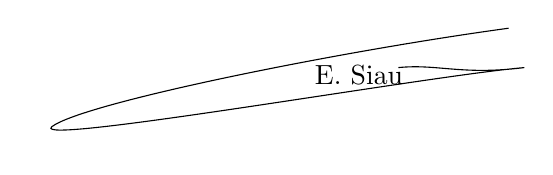
\begin{tikzpicture}[x=1cm,y=1cm]
\draw (5.8,1.25) .. controls (3.6,.95) and (.4,.3) .. (0,0) .. controls (-.3,-.25) and (4.8,.65) .. (6,.75) .. controls (5.2,.65) and (4.9,.8) .. (4.4,.75);
\node at (3.9,.65) {\unsure{E. Siau}};
\end{tikzpicture}}

\uline{E. SIAU}

\margin{137}
